\documentclass[10pt,twocolumn]{article}
\usepackage[utf8]{inputenc}
\usepackage[T1]{fontenc}
\usepackage[margin=0.68in,top=0.72in,bottom=0.75in]{geometry}
\usepackage{amsmath,amssymb}
\usepackage{graphicx}
\usepackage{booktabs}
\usepackage{array}
\usepackage{xcolor}
\usepackage{listings}
\usepackage{caption}
\usepackage[round,authoryear]{natbib}
\usepackage{hyperref}

\definecolor{codebg}{HTML}{F6F8FA}
\definecolor{codeframe}{HTML}{D0D7DE}
\definecolor{codekw}{HTML}{0550AE}
\definecolor{codecmt}{HTML}{57606A}
\definecolor{linkblue}{HTML}{1F4E78}

\hypersetup{
    colorlinks=true,
    linkcolor=linkblue,
    citecolor=linkblue,
    urlcolor=linkblue
}

\captionsetup{font=small,labelfont=bf,skip=4pt}
\emergencystretch=1.5em

\lstset{
    basicstyle=\ttfamily\scriptsize,
    backgroundcolor=\color{codebg},
    frame=single,
    rulecolor=\color{codeframe},
    breaklines=true,
    keywordstyle=\color{codekw}\bfseries,
    commentstyle=\color{codecmt}\itshape,
    showstringspaces=false,
    tabsize=2,
    aboveskip=5pt,
    belowskip=5pt
}

% Dynamically generated statistical macros from Python pipeline
% Auto-generated by paper2_brainimation/generate_figures.py — DO NOT EDIT MANUALLY
\newcommand{\MuseBrowserKB}{19.2}
\newcommand{\BundleReductionFactor}{24.6}
\newcommand{\ERPNoiseRMSKOne}{17.4}
\newcommand{\ERPNoiseRMSKFive}{5.7}
\newcommand{\ERPNoiseRMSKTwenty}{2.7}
\newcommand{\ERPSNRKOne}{0.55}
\newcommand{\ERPSNRKFive}{1.66}
\newcommand{\ERPSNRKTwenty}{3.48}
\newcommand{\EMAVarReductionPct}{98.4}
\newcommand{\NBuiltinExamples}{36}
\newcommand{\NBuiltinCategories}{10}
\newcommand{\NRefAPIs}{94}
\newcommand{\NRefGroups}{22}
\newcommand{\ExLOCMedian}{32}
\newcommand{\ExLOCIQRLow}{27}
\newcommand{\ExLOCIQRHigh}{36}
\newcommand{\ExLOCMin}{11}
\newcommand{\ExLOCMax}{111}
\newcommand{\NStudentSketches}{69}
\newcommand{\NUniqueStudents}{30}
\newcommand{\StuClusterLOCMedian}{164}
\newcommand{\StuClusterLOCIQRLow}{122}
\newcommand{\StuClusterLOCIQRHigh}{173}
\newcommand{\MannWhitneyU}{2437.0}
\newcommand{\MannWhitneyClusterU}{1074.0}
\newcommand{\RankBiserialClusterR}{0.99}
\newcommand{\StuLOCMedian}{155}
\newcommand{\StuLOCMean}{157.5}
\newcommand{\StuLOCSD}{65.7}
\newcommand{\StuLOCIQRLow}{116}
\newcommand{\StuLOCIQRHigh}{189}
\newcommand{\StuLOCMin}{38}
\newcommand{\StuLOCMax}{378}
\newcommand{\NStuNF}{40}
\newcommand{\StuNFLOCMedian}{121}
\newcommand{\StuNFLOCIQRLow}{99}
\newcommand{\StuNFLOCIQRHigh}{171}
\newcommand{\StuNFLOCMin}{38}
\newcommand{\StuNFLOCMax}{378}
\newcommand{\NStuERP}{29}
\newcommand{\StuERPLOCMedian}{176}
\newcommand{\StuERPLOCIQRLow}{153}
\newcommand{\StuERPLOCIQRHigh}{221}
\newcommand{\StuERPLOCMin}{117}
\newcommand{\StuERPLOCMax}{306}
\newcommand{\StuPctCond}{66.7}
\newcommand{\StuCntCond}{46}
\newcommand{\StuPctAlpha}{44.9}
\newcommand{\StuCntAlpha}{31}
\newcommand{\StuPctRaw}{39.1}
\newcommand{\StuCntRaw}{27}
\newcommand{\StuPctBeta}{33.3}
\newcommand{\StuCntBeta}{23}
\newcommand{\StuPctERP}{42.0}
\newcommand{\StuCntERP}{29}
\newcommand{\StuPctAtt}{30.4}
\newcommand{\StuCntAtt}{21}
\newcommand{\StuPctTheta}{23.2}
\newcommand{\StuCntTheta}{16}
\newcommand{\StuPctParticles}{49.3}
\newcommand{\StuCntParticles}{34}
\newcommand{\StuPctMed}{21.7}
\newcommand{\StuCntMed}{15}
\newcommand{\StuPctAudio}{13.0}
\newcommand{\StuCntAudio}{9}
\newcommand{\StuPctEvents}{15.9}
\newcommand{\StuCntEvents}{11}

\raggedbottom

\title{\textbf{BrainImation: A Zero-Install Browser IDE and Creative-Coding Framework for Live WebBluetooth EEG Visualization, Multi-Band Sonification, and Closed-Loop Neurofeedback}}

\author{
\textbf{Kyle E. Mathewson}$^{1,2,*}$\\[4pt]
\footnotesize $^1$Department of Psychology, Faculty of Science, University of Alberta, Edmonton, AB, Canada\\
\footnotesize $^2$Neuroscience and Mental Health Institute, Faculty of Medicine and Dentistry, University of Alberta, Edmonton, AB, Canada\\
\footnotesize $^*$Correspondence: \texttt{kyle.mathewson@ualberta.ca}\\
\footnotesize Live IDE: \url{https://kylemath.github.io/Brainimation/} \ $\cdot$ \ Repository: \url{https://github.com/kylemath/Brainimation}
}

\date{}

\begin{document}
\maketitle

\begin{abstract}
\noindent\textbf{Background:} Authoring custom closed-loop brain--computer interfaces (BCIs), auditory sonifications, and event-related potential (ERP) paradigms with portable electroencephalography (EEG) headsets typically requires complex multi-process desktop toolchains (\texttt{LabStreamingLayer}, Python, C++, or Unity), creating a steep systems-engineering barrier for researchers, educators, and students.\\
\noindent\textbf{New Method:} We present \textsc{BrainImation} (\url{https://kylemath.github.io/Brainimation/}), a zero-install, browser-based live-coding integrated development environment (IDE) that bridges consumer WebBluetooth EEG headsets (InteraXon Muse 2016, Muse~2, and Muse~S) directly with the \texttt{p5.js} 2D/WebGL and \texttt{p5.sound} Web Audio synthesis ecosystems in a single webpage. BrainImation introduces (1) a custom zero-dependency WebBluetooth GATT client (\texttt{muse-browser.js}, \MuseBrowserKB~KB) that resolves the ``lazy GATT characteristic advertisement'' firmware deadlock on Muse~2/S hardware; (2) a dynamic prototype introspection sandbox (\texttt{bindP5Functions}) paired with a dual-source \texttt{window.eegData} state engine (256-sample Hanning-windowed FFT with $>150\ \mu\text{V}$ EOG/EMG rejection and a 256~Hz 4-channel physiological simulator, \texttt{EEGSimulator}); and (3) novice-centered IDE tooling comprising custom Monaco IntelliSense, a \NRefAPIs-API snippet-injecting reference panel, a 440~Hz Web Audio diagnostic engine, and \NBuiltinExamples\ scaffold sketches ($\text{median} = \ExLOCMedian\text{ LOC}$) across \NBuiltinCategories\ categories.\\
\noindent\textbf{Results:} Analytical benchmarks verify Chowning frequency-modulation (FM) Bessel sideband synthesis, $\sqrt{K}$ online 4-channel ERP noise suppression ($\sigma_{\text{noise}}: \ERPNoiseRMSKOne \rightarrow \ERPNoiseRMSKTwenty\ \mu\text{V}$, $\text{SNR}: \ERPSNRKOne \rightarrow \ERPSNRKTwenty$ within $K=20$ trials), and a $\EMAVarReductionPct\%$ reduction in frame-to-frame control jitter via exponential moving-average conditioning. In an empirical human-factors evaluation across $N = \NStudentSketches$ verified code submissions from $N_{\text{students}} = \NUniqueStudents$ novice programmers (\texttt{PSYCH 403}, REB \texttt{Pro00050069}), users expanded the \ExLOCMedian-LOC scaffolds nearly fivefold both across all programs ($\text{median} = \StuLOCMedian\text{ LOC}$, $p < 10^{-15}$) and at the participant-clustered level ($\text{median} = \StuClusterLOCMedian\text{ LOC}$, $p < 10^{-11}$, $r_{rb} = \RankBiserialClusterR$) to author closed-loop neurofeedback games ($N = \NStuNF$, $\text{median} = \StuNFLOCMedian\text{ LOC}$) and online 4-channel ERP paradigms ($N = \NStuERP$, $\text{median} = \StuERPLOCMedian\text{ LOC}$).\\
\noindent\textbf{Comparison with Existing Methods:} Compared to native desktop LSL toolchains (\texttt{BlueMuse}/\texttt{muselsl} + Python) and legacy WebBluetooth bundles (\texttt{muse-js} + \texttt{RxJS}, 473.0~KB), BrainImation reduces compiled BLE client footprint by $\BundleReductionFactor\times$, eliminates Muse~2/S \texttt{NotFoundError} connection crashes, and removes all operating-system driver and inter-process socket dependencies.\\
\noindent\textbf{Conclusions:} BrainImation establishes a reproducible, zero-install browser architecture for rapid prototyping and instruction in closed-loop neurofeedback, brain--computer music interfacing, and online ERP methodology.\\[3pt]
\noindent\textbf{Keywords:} electroencephalography (EEG), brain--computer interface (BCI), WebBluetooth, neurofeedback, event-related potentials (ERPs), open-source software
\end{abstract}

\vspace{2pt}
\noindent\colorbox{codebg}{\parbox{0.97\columnwidth}{\scriptsize\textbf{Highlights ($\le 85$ characters per item):}\\
$\bullet$ Custom 19.2~KB WebBluetooth client fixes Muse 2/S lazy-GATT bug (24.6$\times$ smaller).\\
$\bullet$ Zero-install browser IDE unites 256~Hz EEG, p5.js WebGL, and Web Audio FM synthesis.\\
$\bullet$ Dual-source \texttt{eegData} engine provides 256-pt Hanning FFT and 4-ch 256~Hz simulation.\\
$\bullet$ 94-API snippet reference and 36 scaffolds (median 32~LOC) accelerate BCI authoring.\\
$\bullet$ Validated across 69 BCI and 4-ch ERP programs from 30 novice users ($p < 10^{-11}$).}}
\vspace{4pt}

\section{Introduction}
Closed-loop brain--computer interfaces (BCIs) and neurofeedback systems translate ongoing oscillatory or evoked neural activity into real-time visual, auditory, or mechanical outputs, enabling users to self-regulate cortical states or control interactive applications \citep{sitaram2017closed,enriquez2017eeg,lotte2013flaws}. Beyond clinical rehabilitation, closed-loop EEG holds broad promise for experimental neuroscience, computational media art, and brain--computer music interfacing (BCMI) \citep{miranda2014brain}. Over the past two decades, open-source electrophysiological analysis toolboxes \citep{delorme2004eeglab}, validated portable dry-electrode EEG systems, and single-board acquisition architectures have progressively transitioned electrophysiological recording and analysis outside traditional shielded laboratories \citep{krigolson2017choosing,mathewson2017high,kuziek2017transitioning,kuziek2018increasing}. While browser-based electrophysiology dashboards such as \emph{EEGEdu} (\url{https://eegedu.com}) \citep{mathewson2026eegedu} allow users to inspect live time-domain waveforms, power spectra, and canonical frequency bands through pre-built graphical interfaces, a fundamental methodological bottleneck remains: how can researchers, students, and creative technologists transition from passively observing pre-configured charts to actively programming custom closed-loop neurofeedback environments, audio synthesizers, and online event-related potential (ERP) experiments without a complex multi-language software stack?

\begin{figure*}[t!]
\centering
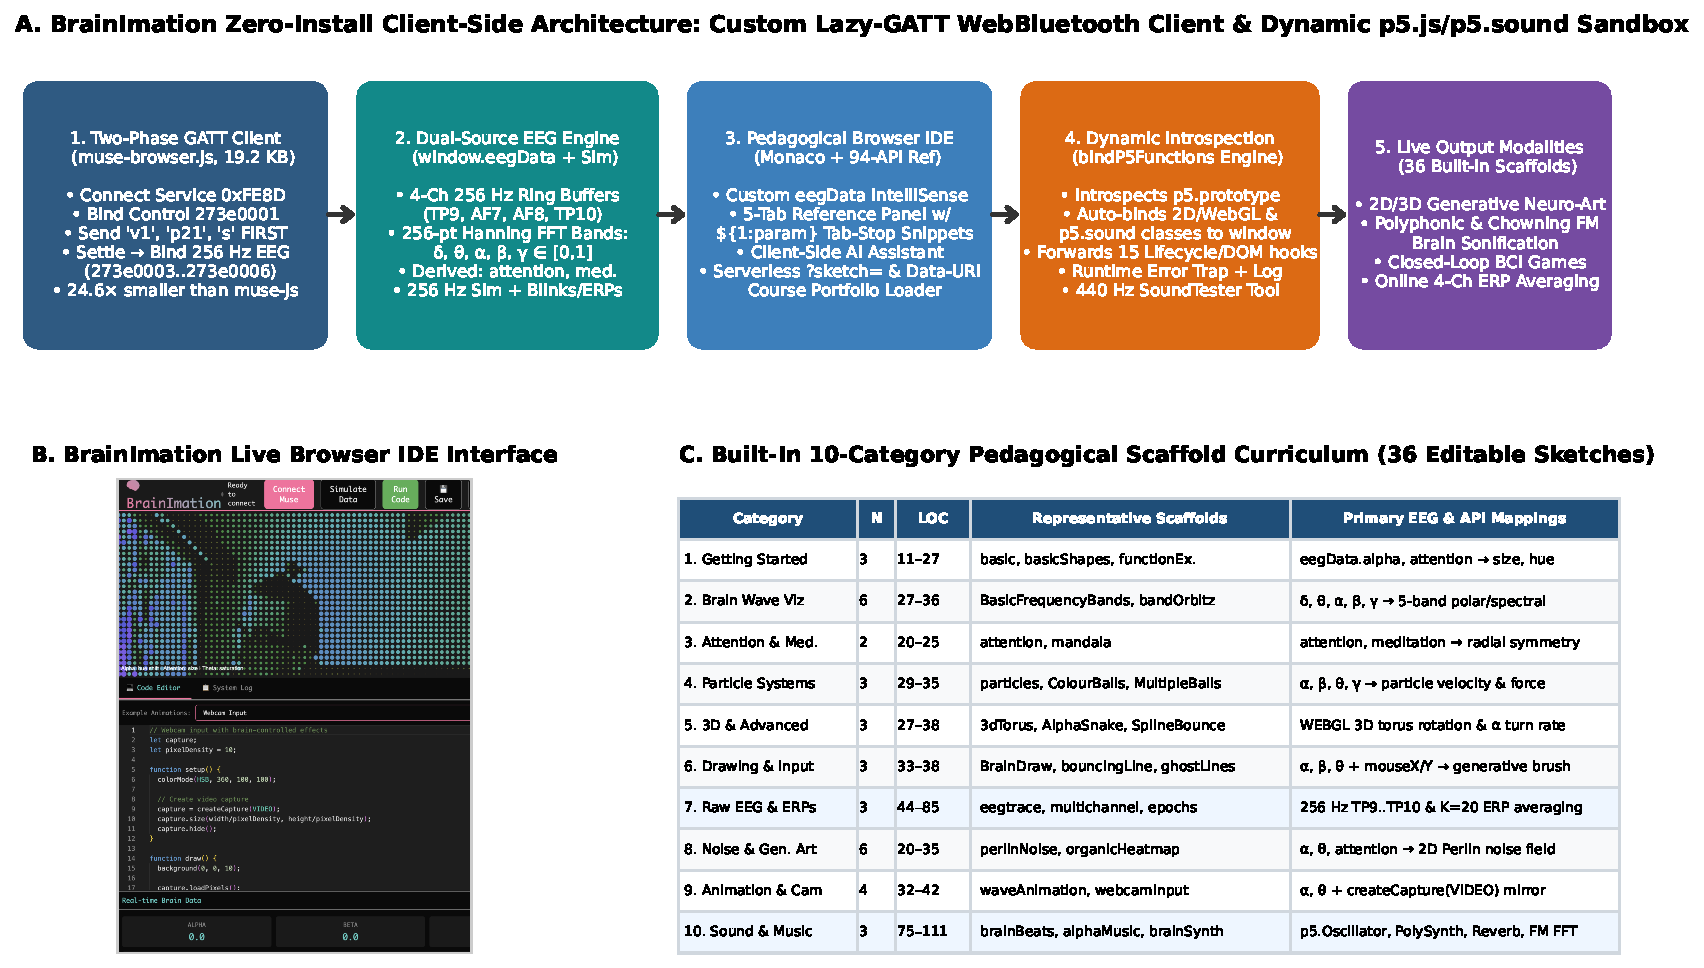
\includegraphics[width=0.98\textwidth]{figures/fig1_brainimation_ide_architecture.pdf}
\caption{\textbf{BrainImation Client-Side Live-Coding Architecture, Two-Phase Lazy-GATT WebBluetooth Protocol, and 10-Category Scaffold Curriculum.} \textbf{(A)} Five-stage architecture spanning the custom \MuseBrowserKB~KB WebBluetooth GATT handshake resolving lazy characteristic advertisement on Muse~2/S firmware, the dual-source 256~Hz 4-channel ring buffer and 256-point Hanning FFT spectral/cognitive state engine (\texttt{window.eegData}) with hardware-free 256~Hz physiological simulation (\texttt{EEGSimulator}), the split-screen VS Code Monaco IDE with custom IntelliSense and 5-tab \NRefAPIs-API click-to-insert snippet reference, the dynamic \texttt{p5.js} and \texttt{p5.sound} prototype introspection runtime (\texttt{bindP5Functions}) with 15 lifecycle and DOM interaction hooks, and 60~FPS visual and Web Audio synthesis output. \textbf{(B)} Live BrainImation browser IDE interface. \textbf{(C)} Taxonomy of the \NBuiltinExamples\ built-in scaffold sketches across \NBuiltinCategories\ progressive pedagogical categories.}
\label{fig:ide}
\end{figure*}

As Seymour Papert's theory of constructionism \citep{papert1980mindstorms} and decades of creative-coding and browser-based experimental design in \texttt{Processing} \citep{reas2007processing}, \texttt{Scratch} \citep{resnick2009scratch}, \texttt{p5.js} \citep{mccarthy2015p5}, and \texttt{jsPsych} \citep{deleeuw2015jspsych} have established, users achieve rapid methodological fluency when environments provide a ``low floor'' (an immediate, frictionless entry point), a ``high ceiling'' (the capacity to build sophisticated, research-grade systems), and ``wide walls'' (support for diverse expressive modalities, from generative art and music to experimental psychology). In conventional BCI workflows, however, the entry floor is prohibitively high. Modulating a simple visual shape or audio oscillator with live alpha waves ($8\text{--}12\text{ Hz}$) typically requires stitching together an operating-system-specific Bluetooth daemon (\texttt{BlueMuse} or \texttt{muse-lsl}), a Lab Streaming Layer (LSL) network socket, a background Python or C++ digital signal processing (DSP) script, and a separate rendering engine such as Unity, PsychoPy, or Max/MSP. Each inter-process boundary introduces cross-platform installation failures, network latency, and hundreds of lines of threading and serialization boilerplate.

Here we eliminate this barrier with \textsc{BrainImation} (\url{https://github.com/kylemath/Brainimation}), a zero-install, single-page browser IDE that unites real-time WebBluetooth electrophysiology with the \texttt{p5.js} and \texttt{p5.sound} creative-coding ecosystems \citep{mccarthy2015p5} (\textbf{Figure~\ref{fig:ide}}). By opening a single URL in Chrome, Edge, or Opera, a user can pair a consumer Muse headband \citep{krigolson2017choosing,kuziek2017transitioning,kuziek2018increasing}---or activate a 256~Hz multi-channel physiological simulator in any modern browser---and author a live closed-loop neurofeedback visualization in just \ExLOCMin~executable lines of JavaScript (\texttt{examples/basic.js}):

\noindent\begin{minipage}{\columnwidth}
\begin{lstlisting}
function setup() {
  colorMode(HSB, 360, 100, 100);
}
function draw() {
  background(0, 0, 10);
  let size = map(eegData.alpha, 0, 1, 50, 300);
  let hue = map(eegData.attention, 0, 1, 180, 360);
  fill(hue, 80, 90);
  noStroke();
  ellipse(width/2, height/2, size, size);
}
\end{lstlisting}
\end{minipage}
\vspace{4pt}

\section{Systems Architecture and Core Engineering Solutions}

\subsection{Solving the Muse 2 / Muse S Lazy-GATT Advertisement Bug and Comparison with Existing Methods}
A primary systems engineering contribution of BrainImation is our custom zero-dependency WebBluetooth client (\texttt{muse-browser.js}; \textbf{Figure~\ref{fig:ide}A} and \textbf{Table~\ref{tab:gatt}}), which eliminates external native LSL daemons while reducing compiled browser bundle size by $\BundleReductionFactor\times$ (\MuseBrowserKB~KB vs.\ 473.0~KB for legacy \texttt{muse-js} + \texttt{RxJS}) and resolving a fatal connection failure mode on modern Muse~2 and Muse~S firmware.

\begin{table}[t!]
\centering
\caption{\textbf{Head-to-Head Comparison of Native Desktop LSL Pipelines, Legacy Browser \texttt{muse-js}, and BrainImation's Two-Phase Client (\texttt{muse-browser.js}).}}
\label{tab:gatt}
\scriptsize
\setlength{\tabcolsep}{2.4pt}
\begin{tabular}{p{0.19\columnwidth}p{0.23\columnwidth}p{0.23\columnwidth}p{0.25\columnwidth}}
\toprule
\textbf{Metric} & \textbf{Desktop LSL (\texttt{muselsl}+Py)} & \textbf{Legacy \texttt{muse-js} (v3.0)} & \textbf{BrainImation (\texttt{muse-browser.js})} \\
\midrule
Install / Deps & OS BLE + Python + LSL & $473.0\text{ KB}$ (\texttt{RxJS}) & \textbf{$\MuseBrowserKB\text{ KB}$ (Zero-Dep, $\BundleReductionFactor\times$ smaller)} \\
GATT Bind & Native BLE daemon & Eager in \texttt{connect()} & \textbf{Two-Phase Lazy Handshake} \\
Muse 2016 & Supported & Partial (PPG crash) & \textbf{100\% Compatible} \\
Muse 2 / Muse S & Fails on Win11 / ChromeOS & Fails (\texttt{NotFoundError}) & \textbf{100\% Compatible} \\
Built-In Sim & None (Hardware req.) & Single-ch mock & \textbf{4-Ch 256~Hz + Blink/ERP Sim} \\
\bottomrule
\end{tabular}
\end{table}

Legacy WebBluetooth wrappers attempt to enumerate and bind the Control characteristic (\texttt{273e0001-4c4d-454d-96be-f03bac821358}) and all four 256~Hz EEG electrode characteristics (\texttt{273e0003} through \texttt{273e0006} for \texttt{TP9}, \texttt{AF7}, \texttt{AF8}, \texttt{TP10}) simultaneously inside \texttt{connect()} immediately upon attaching to primary GATT service \texttt{0xFE8D}. However, diagnostic inspection of newer Muse~2 and Muse~S hardware revealed that modern firmware implements \emph{lazy GATT characteristic advertisement} as a power-saving measure: upon initial connection, only the Control characteristic (\texttt{273e0001}) is exposed in the GATT attribute table. The four EEG data characteristics do not materialize until the host writes a preset selection command (\texttt{"p21"}) and stream-start command (\texttt{"s"}) to \texttt{273e0001}. Eagerly querying \texttt{273e0003..0006} inside \texttt{connect()} therefore triggers a chicken-and-egg deadlock, throwing a fatal \texttt{DOMException: No Characteristics matching UUID found} before \texttt{start()} can ever be called.

Our two-phase initialization protocol in \texttt{muse-browser.js} and \texttt{MuseEEGManager} resolves this hardware race condition deterministically while replacing heavy external reactive dependencies with a lightweight zero-dependency \texttt{SimpleSubject}/\texttt{BehaviorSubject} stream architecture:
\begin{lstlisting}
// Phase 1 (connect): Bind ONLY Control characteristic (273e0001)
this.controlChar = await this.service.getCharacteristic(CONTROL_CHAR_UUID);
await this.controlChar.startNotifications();

// Phase 2 (start): Wake firmware, set preset, and trigger GATT exposure
await this.pause();            // Halt residual stream ('h')
await this.delay(100);
await this.sendCommand('v1');  // Query firmware version
await this.delay(100);
await this.sendCommand('p21'); // Select 4-ch EEG preset (safe on Muse 2016)
await this.delay(100);
await this.sendCommand('s');   // Start streaming -> exposes EEG UUIDs
await this.delay(100);
await this.resume();           // Resume stream ('d')
await this.delay(500);         // Settle delay for GATT table update

// Discover and bind 256 Hz EEG characteristics (273e0003..0006)
const allChars = await this.service.getCharacteristics();
\end{lstlisting}
Length-prefixed ASCII control commands are serialized via \texttt{encodeCommand(cmd)} as \texttt{[cmd.length + 1, ...charCodes, 0x0a]}. Incoming 20-byte BLE notification packets (containing a 16-bit unsigned packet sequence index followed by twelve packed 12-bit unsigned offset-binary samples at $f_s = 256\text{ Hz}$) are unpacked via bitwise shift-and-mask operations in \texttt{decodeEEGSamples()} and scaled to microvolts centered at mid-scale ($2048 = \texttt{0x800}$):
\begin{equation}
V_{i} = 0.48828125 \times \left( s_{i} - 2048 \right) \ \mu\text{V}, \qquad i \in \{0, \dots, 11\}.
\end{equation}

\subsection{Dual-Source Signal Abstraction (\texttt{window.eegData}), 256-Point Hanning FFT, and 256~Hz Simulator (\texttt{EEGSimulator})}
To guarantee that student code executes identically whether connected to a physical Muse headband in the teaching laboratory or developed offline on a personal laptop at home, \texttt{MuseEEGManager} and \texttt{EEGSimulator} both populate a unified global state object, \texttt{window.eegData}. This object exposes three complementary tiers of real-time neural data.

At the spectral level, \texttt{MuseEEGManager.\allowbreak calculateFrequencyBands()} computes normalized frequency bands scaled to $[0.0, 1.0]$---\texttt{eegData.delta} ($1\text{--}4\text{ Hz}$), \texttt{eegData.theta} ($4\text{--}8\text{ Hz}$), \texttt{eegData.alpha} ($8\text{--}12\text{ Hz}$), \texttt{eegData.beta} ($13\text{--}30\text{ Hz}$), and \texttt{eegData.gamma} ($30\text{--}50\text{ Hz}$)---from sliding $N = 256$-sample ($1.0\text{ s}$ at $f_s = 256\text{ Hz}$, yielding a Rayleigh frequency bin resolution of $\Delta f = f_s / N = 1.0\text{ Hz}$) electrode windows across \texttt{TP9}, \texttt{AF7}, \texttt{AF8}, and \texttt{TP10}. For each channel $c$, the DC mean $\bar{x}_c$ is subtracted and the centered window is screened for gross ocular (EOG) or frontalis/temporalis myogenic (EMG) artifacts; any channel window exceeding $\max_{n} |x_c[n] - \bar{x}_c| > 150\ \mu\text{V}$ is rejected before spectral estimation so that eye blinks or jaw clenches do not masquerade as oscillatory band power. Artifact-free windows are tapered with a 256-point Hanning window, $w[n] = 0.5\big(1 - \cos(2\pi n / (N - 1))\big)$, and transformed via an in-place radix-2 Cooley--Tukey FFT (\texttt{computeRadix2FFT()}) to obtain single-sided power spectral density estimates $P_c[k] = (2 / N^2)\big(\text{Re}(X_c[k])^2 + \text{Im}(X_c[k])^2\big)$ at integer frequencies $k \in \{1, \dots, 50\}\text{ Hz}$. Band powers are averaged across valid electrodes, weighted by $1/f$ compensation gains ($w_b \in \{0.35, 0.75, 1.00, 2.20, 4.00\}$ for $\delta, \theta, \alpha, \beta, \gamma$) to equalize canonical dynamic ranges, and normalized by total weighted broadband power into $[0.0, 1.0]$. At the cognitive-state level, \texttt{window.eegData} computes composite indices in $[0.0, 1.0]$ for \texttt{eegData.attention} via $(\beta + \gamma)/2$ and \texttt{eegData.meditation} via $(\alpha + \theta)/2$. At the sample level, it maintains 256~Hz multi-channel time-series ring buffers, including \texttt{eegData.raw} (instantaneous 4-element vector in $\mu\text{V}$), \texttt{eegData.rawHistory} (1,000-sample rolling FIFO queues per channel), \texttt{eegData.getRawChannel(ch, N)}, \texttt{eegData.getAllChannels(N)}, and \texttt{eegData.\allowbreak getRecentEpoch(N)}, which returns a transposed $N \times 4$ sample-by-electrode matrix for online ERP epoching.

When a learner clicks \texttt{Simulate Data}, \texttt{EEGSimulator} (\textbf{Figure~\ref{fig:scaffolding}B}) reveals interactive Attention ($A_0 \in [0,1]$) and Meditation ($M_0 \in [0,1]$) sliders in the IDE sidebar, pre-populates $1.0\text{ s}$ (256 samples) of history, and streams 8 samples every $31.25\text{ ms}$ (maintaining an exact $f_s = 256\text{ Hz}$ multi-channel sampling rate). For each electrode $c \in \{0,1,2,3\}$ (\texttt{TP9}, \texttt{AF7}, \texttt{AF8}, \texttt{TP10}), microvolt time series $V_c(t)$ at $t = n / 256\text{ s}$ are synthesized as a multi-band oscillatory superposition with slow baseline drift, broadband sensor noise, bilateral anterior frontal eye-blink artifacts, and optional stimulus-locked ERP waveforms:
\begin{align}
V_c(t) &= 30\alpha(t)\sin\!\big(2\pi(9 + 0.5c)t\big) \nonumber\\
&\quad + 20\beta(t)\sin\!\big(2\pi(18 + 1.5c)t\big) \nonumber\\
&\quad + 25\theta(t)\sin\!\big(2\pi(6 + 0.3c)t\big) \nonumber\\
&\quad + 40\delta(t)\sin\!\big(2\pi(2 + 0.2c)t\big) \nonumber\\
&\quad + 10\gamma(t)\sin\!\big(2\pi(35 + 2c)t\big) + 5\sin(2\pi \cdot 0.1t) \nonumber\\
&\quad + \eta_c(t) + \mathbb{I}_{c \in \{1,2\}} B(t) + E_{\text{ERP}}(t),
\end{align}
where $\eta_c(t) \sim \mathcal{U}(-7.5, 7.5)\ \mu\text{V}$ models broadband sensor noise, $\mathbb{I}_{c \in \{1,2\}} B(t)$ injects synchronous bilateral Gaussian ocular blink deflections ($B(t) = 115\exp(-(t - t_{\text{blink}})^2 / (2\sigma_b^2))\ \mu\text{V}$, $\sigma_b = 25\text{ ms}$) onto the anterior frontal channels (\texttt{AF7}, \texttt{AF8}) with Bernoulli probability $p = 0.001$ per sample (\textbf{Figure~\ref{fig:scaffolding}B}), and $E_{\text{ERP}}(t)$ injects time-locked N170 ($-6.5\ \mu\text{V}$ at $+170\text{ ms}$) and P300 ($+9.5\ \mu\text{V}$ at $+340\text{ ms}$) components whenever a sketch invokes \texttt{eegData.triggerERP()}.

\subsection{Dynamic Prototype Introspection and Lifecycle Sandbox (\texttt{bindP5Functions})}
Embedding a live-reloading \texttt{p5.js} execution environment inside a multi-panel web application poses a major architectural conflict. Standard \texttt{p5.js} ``global mode'' binds functions once on page load and cannot cleanly tear down and re-initialize canvases and Web Audio nodes on repeated \texttt{Run Code} clicks. Conversely, ``instance mode'' (\texttt{new p5(p => \{...\})}) isolates canvas lifecycles but forces students to prefix every function call with \texttt{p.} (\texttt{p.ellipse()}, \texttt{p.map()}), breaking compatibility with standard \texttt{p5.js} tutorials. Furthermore, manually binding a static list of drawing functions fails to expose addon libraries such as \texttt{p5.sound}.

BrainImation resolves this via dynamic prototype introspection (\texttt{bindP5Functions()} in \texttt{CodeEditor.runCode()}). Whenever a sketch runs, BrainImation destroys the prior \texttt{p5} instance, instantiates a fresh sandbox attached to \texttt{\#canvas-container}, and iterates over all enumerable and prototype properties of the instance (\texttt{for (let prop in p)}), automatically binding every method to \texttt{window} while copying mathematical and rendering constants (\texttt{PI}, \texttt{TWO\_PI}, \texttt{HSB}, \texttt{WEBGL}) and exposing all \texttt{p5.sound} synthesis classes (\texttt{p5.Oscillator}, \texttt{p5.PolySynth}, \texttt{p5.MonoSynth}, \texttt{p5.FFT}, \texttt{p5.Amplitude}, \texttt{p5.Reverb}, \texttt{p5.Delay}, \texttt{p5.Filter}). The sandbox then evaluates the student's code in global scope, captures up to 15 user-defined lifecycle and interaction hooks (the 2 core lifecycle hooks \texttt{setup} and \texttt{draw}, plus 13 DOM/input hooks: \texttt{windowResized}, \texttt{mousePressed}, \texttt{mouseReleased}, \texttt{mouseClicked}, \texttt{mouseMoved}, \texttt{mouseDragged}, \texttt{mouseWheel}, \texttt{keyPressed}, \texttt{keyReleased}, \texttt{keyTyped}, \texttt{touchStarted}, \texttt{touchMoved}, and \texttt{touchEnded}), and synchronizes dynamic system variables (\texttt{frameCount}, \texttt{mouseX}, \texttt{mouseY}, \texttt{key}, \texttt{keyCode}, \texttt{touches}) on every animation frame. If a runtime exception occurs inside \texttt{draw()}, the sandbox catches the error, halts the animation loop via \texttt{p.noLoop()} to prevent console flooding, extracts the offending line number from the stack trace, and prints an actionable debugging hint to the in-app System Log (\texttt{ConsoleLogger}).

\begin{figure*}[t!]
\centering
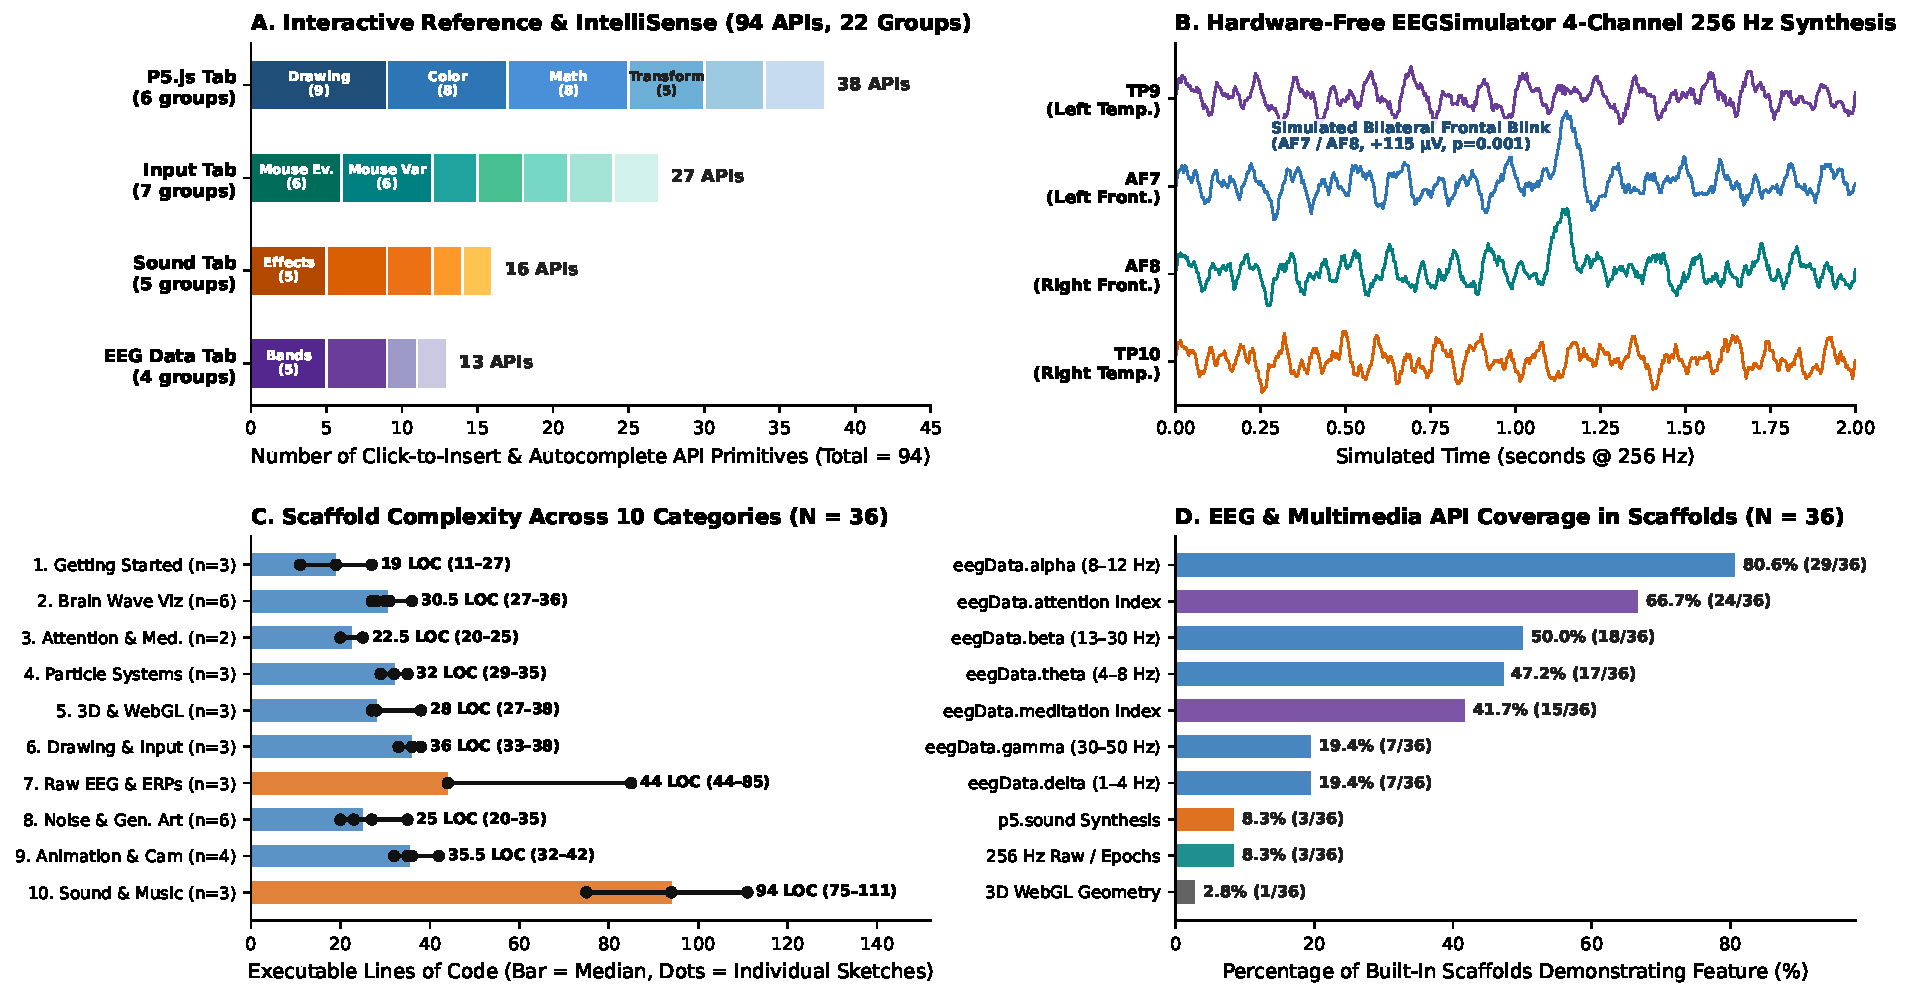
\includegraphics[width=0.98\textwidth]{figures/fig2_ide_scaffolding_and_corpus.pdf}
\caption{\textbf{Pedagogical IDE Scaffolding, \NRefAPIs-Primitive Interactive Reference Database, Hardware-Free 256~Hz Multi-Channel Simulation, and 10-Category Scaffold Profile.} \textbf{(A)} Distribution of the \NRefAPIs\ curated API primitives across \NRefGroups\ functional groups and 4 reference tabs (\texttt{P5.js}, \texttt{Input}, \texttt{Sound}, and \texttt{EEG Data}) that power both Monaco IntelliSense autocomplete and regex-parsed \texttt{\$\{1:param\}} tab-stop snippet insertion. \textbf{(B)} Two-second 4-channel (\texttt{TP9}, \texttt{AF7}, \texttt{AF8}, \texttt{TP10}) synthetic 256~Hz microvolt traces generated by \texttt{EEGSimulator}, illustrating multi-band oscillatory superposition and synchronous bilateral anterior frontal (\texttt{AF7}/\texttt{AF8}) eye-blink artifacts. \textbf{(C)} Executable Lines of Code (LOC) across the \NBuiltinCategories\ built-in pedagogical categories ($N = \NBuiltinExamples$ sketches; bars show category median, horizontal lines span min--max range, and dots show individual sketches). \textbf{(D)} Percentage of the \NBuiltinExamples\ built-in scaffolds demonstrating each \texttt{eegData} and multimedia capability.}
\label{fig:scaffolding}
\end{figure*}

\section{Pedagogical IDE Scaffolding, Reference Tooling, and Serverless Portfolio Workflow}

\subsection{Context-Aware Monaco Autocomplete and Snippet-Injecting Reference Panel}
To minimize syntactic friction for psychology and neuroscience students who have never written JavaScript, BrainImation pairs Microsoft's VS Code Monaco editor with two synchronized code-discovery engines (\textbf{Figure~\ref{fig:scaffolding}A}). First, using \texttt{monaco.languages.registerCompletionItemProvider}, the editor provides context-aware \texttt{eegData} and \texttt{p5} IntelliSense by inspecting the token preceding the cursor on every keystroke. Typing \texttt{eegData.} filters the completion menu exclusively to the 13 EEG properties and ring-buffer methods (complete with live type signatures and docstrings), whereas general typing surfaces all \NRefAPIs\ curated API primitives across drawing, color, math, Web Audio synthesis, and user input. Second, a collapsible right-hand drawer (\texttt{ReferencePanel}) organizes the \NRefAPIs\ primitives into \NRefGroups\ groups across four documentation tabs---\emph{P5.js} (38 primitives across Drawing [9], Color [8], Math [8], Transform [5], Control [4], and Text [4]), \emph{Input} (27 primitives across Mouse Events [6], Mouse Variables [6], Keyboard Events [3], Keyboard Variables [3], Touch Events [3], Touch Variables [3], and Interactive Templates [3]), \emph{Sound} (16 primitives across Effects [5], Control [4], Synthesizers [3], Sound Files [2], and Spectral Analysis [2]), and \emph{EEG Data} (13 primitives across Frequency Bands [5], Raw Data Access [4], Derived Metrics [2], and Connection Status [2])---plus a fifth \emph{AI Helper} tab. Clicking any item expands its signature and description, while clicking a second time invokes \texttt{ReferencePanel.createSnippet()}, which parses the function signature via regular expressions to strip optional brackets and synthesize numbered Monaco tab-stop placeholders:
\begin{lstlisting}
// Signature: "ellipse(x, y, width, [height])"
// Synthesized Monaco snippet injected via snippetController2:
ellipse(${1:x}, ${2:y}, ${3:width}, ${4:height})
\end{lstlisting}
Injecting this template via Monaco's \texttt{snippetController2} places the student's cursor directly inside the first argument and allows them to press \texttt{Tab} to step sequentially through each required parameter.

\subsection{Web Audio Diagnostic Synthesizer (\texttt{SoundTester}) and Client-Side AI Assistant (\texttt{AIAssistant})}
Modern web browsers enforce strict autoplay policies that suspend the Web Audio \texttt{AudioContext} until a user gesture occurs on the page. When a student's first sonification sketch fails to produce sound, novices struggle to determine whether the bug lies in their JavaScript code, a suspended browser \texttt{AudioContext}, or muted OS hardware. BrainImation therefore includes a dedicated \texttt{Test Sound} diagnostic engine (\texttt{SoundTester}) in the top toolbar that executes a five-stage automated verification in the System Log, checking CDN availability of \texttt{p5.Oscillator}, verifying browser \texttt{AudioContext} support, inspecting and explicitly resuming any \texttt{suspended} audio context via \texttt{userStartAudio()}, bypassing user code to instantiate an isolated 440~Hz (\texttt{A4}) sine-wave reference oscillator, and ramping envelope amplitude to $0.3$ for $1.0\text{ s}$ with step-by-step pass/fail telemetry.

For students who wish to explore natural-language code generation or automated debugging, the fifth tab of the reference drawer hosts a privacy-preserving, client-side AI Code Assistant (\texttt{AIAssistant}). Students can optionally supply their own OpenAI (\texttt{gpt-4}) or Anthropic (\texttt{claude-3-5-sonnet}) API key, which is stored strictly in browser \texttt{localStorage} and never transmitted to any intermediary server. When invoked, \texttt{AIAssistant} constructs a domain-specific system prompt containing the complete \texttt{window.eegData} specification alongside the student's current Monaco editor buffer, strips markdown fences from the returned code, loads the generated program into the editor, and automatically executes it on the live EEG stream.

\subsection{Serverless URL Sketch Loading (\texttt{?sketch=}) and Course Portfolio Pipeline}
To support classroom instruction and grading without requiring database servers or student user accounts, \texttt{CodeEditor.checkAndLoadFromURL()} implements a serverless code-sharing protocol via URL query parameters (\texttt{?sketch=} or \texttt{?code=}, plus optional \texttt{\&autorun=true}). Through remote file and cloud portfolio links, instructors and automated course portfolio generators can link directly to student \texttt{.js} or \texttt{.txt} code submissions hosted on Google Drive, GitHub, or course websites (e.g., \texttt{?code=https://.../part2.txt\&autorun=true}). Crucially, \texttt{checkAndLoadFromURL()} is sequenced inside the Monaco AMD loader callback \emph{prior} to default sketch initialization, preventing race conditions between asynchronous network fetches and default code execution. Alternatively, sketches can be encoded entirely inside the URL as self-contained Base64 Data URIs (\texttt{?sketch=data:text/plain;base64,...}), enabling zero-storage, offline-capable sharing of complete neurofeedback programs in a single hyperlink.

\subsection{The 10-Category Pedagogical Scaffold Curriculum (\NBuiltinExamples\ Built-In Sketches)}
Rather than confronting learners with an empty editor, BrainImation provides a manifest-driven library of \NBuiltinExamples\ built-in example sketches organized across \NBuiltinCategories\ progressive categories (\textbf{Figure~\ref{fig:ide}C} and \textbf{Figure~\ref{fig:scaffolding}C,D}). Each example is a standalone \texttt{.js} file in \texttt{examples/} headed by a lightweight JSDoc metadata block (\texttt{@id}, \texttt{@title}, \texttt{@category}, \texttt{@order}) that is parsed dynamically at runtime by \texttt{loadExampleAnimations()}. Across all \NBuiltinExamples\ scaffolds, executable code length has a median of just \ExLOCMedian~LOC ($\text{IQR} = \ExLOCIQRLow\text{--}\ExLOCIQRHigh\text{ LOC}$, range $\ExLOCMin\text{--}\ExLOCMax\text{ LOC}$; \textbf{Figure~\ref{fig:scaffolding}C}), establishing a low-floor entry point across every creative modality.

In the introductory categories (Categories 1--3: Introductory Mapping, Spectral Dashboards, and Mindfulness; $n = 11$, $11\text{--}36\text{ LOC}$), sketches progress from \texttt{basic.js} (11~LOC) and \texttt{basicShapes.js} (19~LOC) to 5-band polar and orbital visualizers (\texttt{bandOrbitz.js}, \texttt{piWedges.js}, \texttt{spectra.js}) and meditation-driven geometric mandalas (\texttt{mandala.js}, 25~LOC). The intermediate visual and interactive categories (Categories 4--6 and 8--9: Particles, 3D WebGL, Generative Noise, and Webcam Interaction; $n = 19$, $20\text{--}42\text{ LOC}$) demonstrate multi-agent particle physics (\texttt{particles.js}, \texttt{MultipleBalls.js}), 3D WebGL hardware-accelerated geometry (\texttt{3dTorus.js}, 28~LOC), closed-loop steering (\texttt{AlphaSnake.js}, 27~LOC), mind-controlled brush painting (\texttt{BrainDraw.js}, 36~LOC), multi-octave 2D Perlin flow fields (\texttt{perlinNoise.js}, \texttt{noiseDetail.js}), and live webcam video mirroring modulated by alpha and theta oscillations (\texttt{webcamInput.js}, 42~LOC). Finally, Categories 7 and 10 (Raw 256~Hz Time-Series, Online ERPs, and Web Audio Sonification; $n = 6$, $44\text{--}111\text{ LOC}$) provide advanced research and musical synthesis templates, which we detail in Section~4.

\begin{figure*}[t!]
\centering
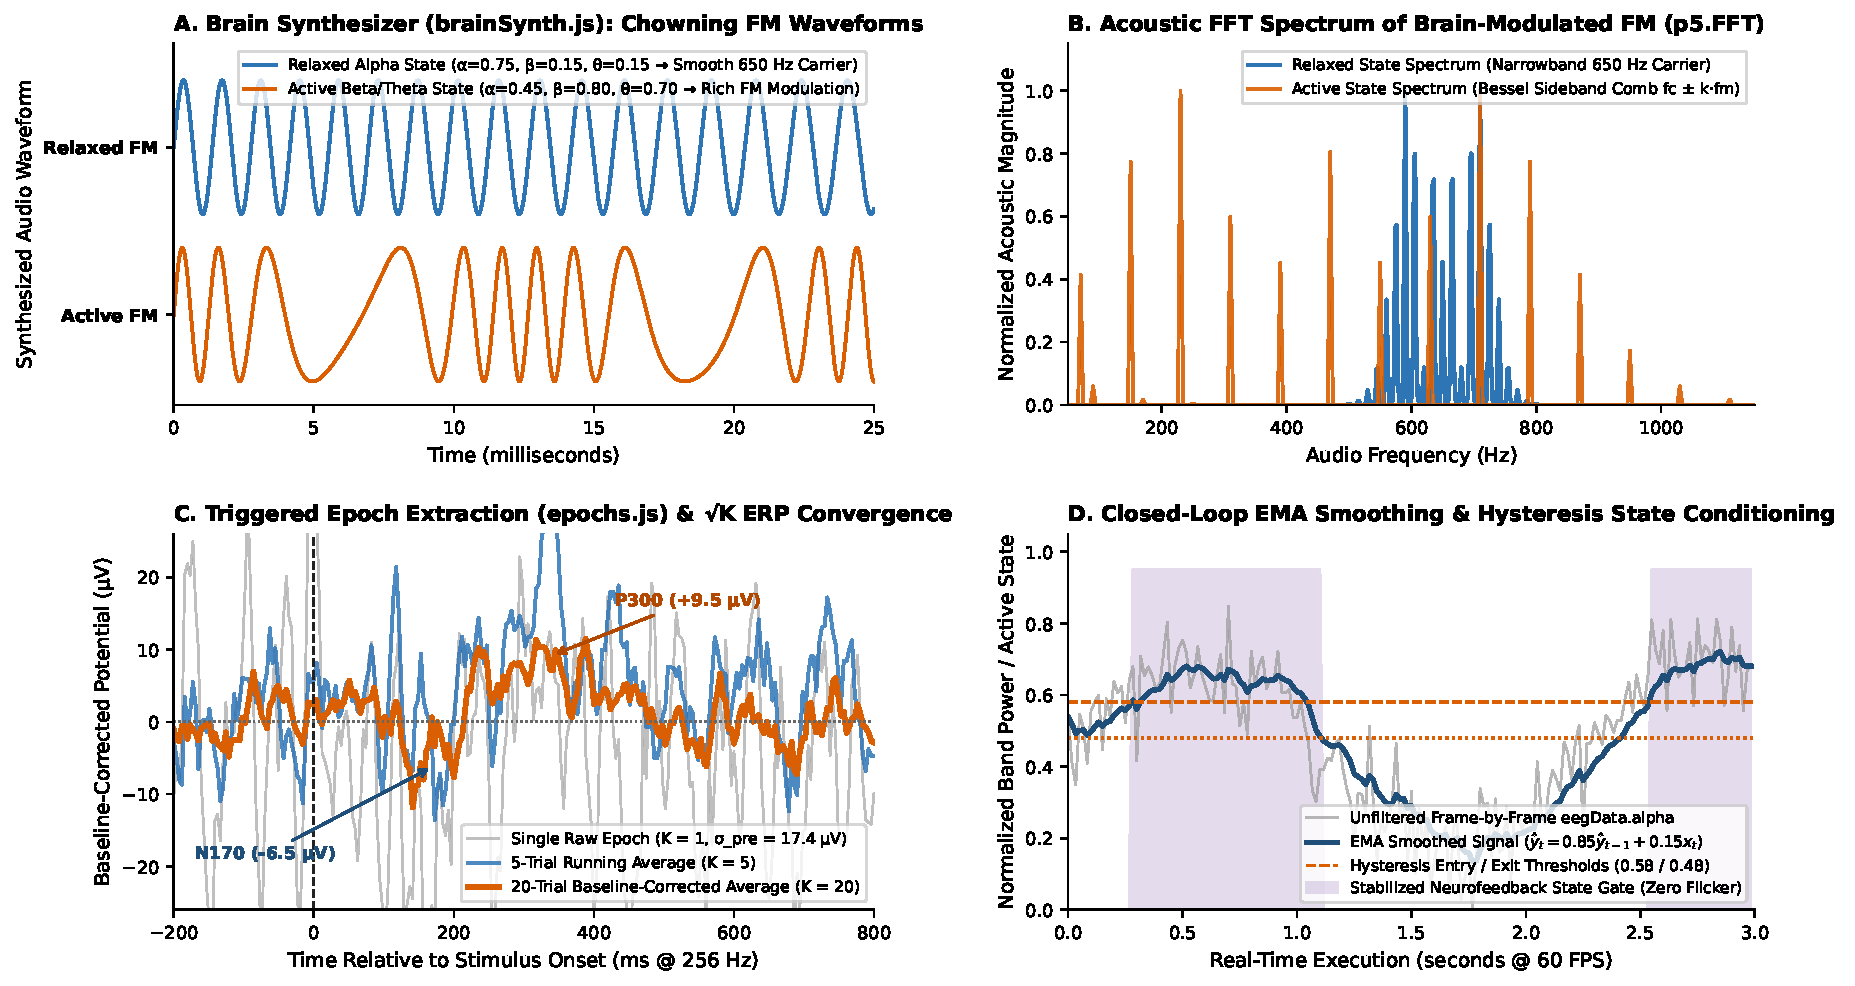
\includegraphics[width=0.98\textwidth]{figures/fig3_sonification_and_erp_engine.pdf}
\caption{\textbf{Multi-Band Web Audio FM Sonification, Online 4-Channel ERP Grand Averaging, and Closed-Loop Signal Conditioning.} \textbf{(A)} Synthesized time-domain audio waveforms in \texttt{brainSynth.js} comparing a relaxed high-alpha state ($\alpha=0.75, \beta=0.15, \theta=0.15 \rightarrow 650\text{ Hz}$ smooth carrier) against an active high-beta/theta state ($\alpha=0.45, \beta=0.80, \theta=0.70 \rightarrow 470\text{ Hz}$ carrier with $80\text{ Hz}$ modulator and $350\text{ Hz}$ deviation). \textbf{(B)} Corresponding acoustic FFT magnitude spectra (\texttt{p5.FFT}) showing narrowband harmonic output during relaxation vs.\ wide Bessel sideband combs ($f_c \pm k f_m$) during active beta/theta engagement. \textbf{(C)} Triggered online 256~Hz epoch extraction via \texttt{eegData.getRecentEpoch(256)} ($-200\text{ to }+800\text{ ms}$, $L_{\text{pre}} = 51$ baseline samples) and $\sqrt{K}$ background noise reduction across $K = 1, 5,$ and $20$ averaged trials in \texttt{epochs.js}, revealing time-locked N170 ($-6.5\ \mu\text{V}$) and P300 ($+9.5\ \mu\text{V}$) deflections. \textbf{(D)} Closed-loop exponential moving average (EMA) smoothing ($\hat{y}_t = 0.85\hat{y}_{t-1} + 0.15x_t$) and dual-threshold hysteresis gating used in student neurofeedback applications to eliminate single-frame threshold chatter.}
\label{fig:sonification}
\end{figure*}

\section{Multi-Band Sonification, Online ERP Averaging, and Closed-Loop Signal Conditioning}

\subsection{Real-Time Web Audio Sonification and Chowning FM Synthesis}
BrainImation brings real-time brain--computer music interfacing (BCMI) directly into the browser without external audio middleware (\textbf{Figure~\ref{fig:sonification}A,B}). Three progressive scaffolds in the \emph{Sound \& Music} category illustrate how continuous, FFT-derived neural metrics can drive Web Audio synthesis graphs. The introductory sonification sketch (\texttt{brainBeats.js}, 75~LOC) maps \texttt{eegData.alpha} linearly to the fundamental frequency of a sine-wave oscillator ($f_0 \in [200, 800]\text{ Hz}$) and \texttt{eegData.beta} to acoustic amplitude, providing immediate eyes-closed alpha auditory neurofeedback. Building on this, \texttt{alphaMusic.js} (94~LOC) implements generative pentatonic polyphony with convolution reverb by routing a polyphonic synthesizer (\texttt{p5.PolySynth}) through a 3-second digital reverb (\texttt{p5.Reverb}); normalized \texttt{alpha} quantizes pitch selection onto a 6-note C-major pentatonic scale ($\{\text{C}_4, \text{D}_4, \text{E}_4, \text{G}_4, \text{A}_4, \text{C}_5\}$; $261.63\text{--}523.25\text{ Hz}$), \texttt{attention} modulates millisecond inter-onset note tempo via \texttt{millis()} ($200\text{--}800\text{ ms}$), \texttt{meditation} scales note velocity ($0.3\text{--}1.0$), and \texttt{beta} controls note sustain duration ($0.1\text{--}0.5\text{ s}$). The most advanced audio scaffold (\texttt{brainSynth.js}, 111~LOC; \textbf{Figure~\ref{fig:sonification}A,B}) constructs a four-dimensional Chowning frequency-modulation (FM) synthesizer with live spectral analysis by disconnecting a sinusoidal modulator oscillator from the master output (\texttt{modulator.disconnect()}) and patching it directly into the frequency control node of a carrier oscillator (\texttt{carrier.freq(modulator)}) while analyzing the resulting acoustic output via \texttt{new p5.FFT()} \citep{chowning1973synthesis,mccarthy2015p5}:
\begin{equation}
s(t) = A(\text{att}) \sin\!\left( 2\pi f_{c}(\alpha)\, t + \frac{\Delta f(\theta)}{f_{m}(\beta)} \sin\!\big(2\pi f_{m}(\beta)\, t\big) \right),
\end{equation}
where \texttt{alpha} controls carrier pitch $f_c(\alpha) = 200 + 600\alpha\text{ Hz}$, \texttt{beta} drives modulation frequency $f_m(\beta) = 100\beta\text{ Hz}$, \texttt{theta} governs modulation depth $\Delta f(\theta) = 500\theta\text{ Hz}$ (controlling the modulation index $I = \Delta f / f_m$), and \texttt{attention} scales master envelope gain $A \in [0, 0.2]$ using a $100\text{ ms}$ Web Audio slew-rate ramp time constant (\texttt{carrier.amp(volume, 0.1)}) to prevent 60~Hz frame-boundary clicks (``zipper noise''). As shown in \textbf{Figure~\ref{fig:sonification}A,B}, a relaxed high-alpha state produces a pure, warm $650\text{ Hz}$ sinusoidal tone, whereas elevated beta and theta activity dynamically expands the modulation index, generating a rich comb of acoustic Bessel sidebands at $f_c \pm k f_m$ rendered in real time on the canvas spectrum analyzer.

\subsection{Multi-Channel 256~Hz Oscilloscopes and Online ERP Grand Averaging (\texttt{epochs.js})}
While spectral sketches consume normalized band powers, the \emph{Raw EEG Data} category exposes the underlying 256~Hz microvolt time series across \texttt{TP9}, \texttt{AF7}, \texttt{AF8}, and \texttt{TP10}. \texttt{eegtrace.js} (44~LOC) and \texttt{multichannel.js} (44~LOC) call \texttt{eegData.getRawChannel(ch, 256)} to render scrolling 4-channel microvolt oscilloscopes. Building on this, \texttt{epochs.js} (85~LOC; \textbf{Figure~\ref{fig:sonification}C}) implements triggered online event-related potential (ERP) ensemble averaging \citep{luck2014introduction,krigolson2017choosing}. Every 90 animation frames ($\sim 1.5\text{ s}$), the sketch presents a visual stimulus flash on canvas at $t = 0\text{ ms}$ (and invokes \texttt{eegData.triggerERP('target')} when running on \texttt{EEGSimulator}). Because \texttt{eegData.getRecentEpoch(L)} retrieves the most recent $L$ samples from the rolling 256~Hz FIFO ring buffer, the sketch waits 48 frames ($+800\text{ ms} = 205\text{ post-stimulus samples}$ after stimulus onset) before calling \texttt{eegData.getRecentEpoch(256)}. This causal post-stimulus capture extracts the complete $L = 256$-sample ($1,000\text{ ms}$) epoch matrix $\mathbf{E}^{(k)} \in \mathbb{R}^{256 \times 4}$ spanning $-200\text{ ms}$ ($L_{\text{pre}} = 51$ pre-stimulus baseline samples) through $+800\text{ ms}$ ($205$ post-stimulus samples). The sketch then subtracts the pre-stimulus baseline mean across samples $j \in \{0, \dots, L_{\text{pre}}-1\}$ for each electrode $c$ and updates the running grand average across $K$ trials:
\begin{equation}
\widehat{\text{ERP}}_{c}(t_i) = \frac{1}{K} \sum_{k=1}^{K} \left( E^{(k)}_{i,c} - \frac{1}{L_{\text{pre}}} \sum_{j=0}^{L_{\text{pre}}-1} E^{(k)}_{j,c} \right).
\end{equation}
Because ongoing background EEG oscillations ($\sigma_0 = \ERPNoiseRMSKOne\ \mu\text{V}$ baseline RMS on a single trial) are phase-independent across stimulus repetitions, ensemble averaging suppresses non-phase-locked noise by $\sigma_{\text{noise}}(K) = \sigma_0 / \sqrt{K}$ (\textbf{Figure~\ref{fig:sonification}C}), reducing pre-stimulus baseline RMS noise from $\ERPNoiseRMSKOne\ \mu\text{V}$ ($K=1$, P300 $\text{SNR} = \ERPSNRKOne$) to $\ERPNoiseRMSKFive\ \mu\text{V}$ at $K=5$ ($\text{SNR} = \ERPSNRKFive$) and $\ERPNoiseRMSKTwenty\ \mu\text{V}$ at $K=20$ ($\text{SNR} = \ERPSNRKTwenty$), allowing time-locked sensory and cognitive components (such as the visual N170 and oddball P300) to emerge clearly on screen within 20 trials.

\subsection{Closed-Loop Signal Conditioning for Interactive Neurofeedback}
When continuous EEG metrics drive interactive games or state classifiers at 60~FPS, raw frame-to-frame spectral estimates exhibit finite-window variance that can cause visual jitter or rapid ``threshold flicker'' \citep{lotte2013flaws}. Within BrainImation, this challenge serves as an explicit methodological pattern in closed-loop control engineering (\textbf{Figure~\ref{fig:sonification}D}): users condition raw \texttt{eegData} streams using first-order exponential moving-average (EMA) filters,
\begin{equation}
\hat{y}_{t} = \lambda \hat{y}_{t-1} + (1 - \lambda) x_{t}, \qquad \lambda \in [0.80, 0.95],
\end{equation}
which reduces frame-to-frame first-difference variance $\text{Var}(\Delta \hat{y}_t)$ by $\EMAVarReductionPct\%$ at $\lambda = 0.85$ (\textbf{Figure~\ref{fig:sonification}D}), paired with dual-threshold Schmitt-trigger hysteresis gates ($T_{\text{enter}} > T_{\text{exit}}$) or minimum dwell-time counters (\texttt{holdFrames}) that eliminate transient single-frame state chatter.

\section{Empirical Programmability and Human-Factors Validation (\texorpdfstring{$N = \NStudentSketches$}{N = \NStudentSketches} Applications from \texorpdfstring{$N_{\text{students}} = \NUniqueStudents$}{N\_students = \NUniqueStudents} Novice Developers)}

\begin{table*}[t!]
\centering
\caption{\textbf{Quantitative Comparison of Code Complexity and Verified Executable EEG Feature Adoption Across BrainImation's Built-In Scaffolds and $N = \NStudentSketches$ Undergraduate Student Submissions ($N_{\text{students}} = \NUniqueStudents$ Unique Learners in \texttt{PSYCH 403}).} Metrics are extracted directly from executable source lines via \texttt{paper2\_brainimation/generate\_figures.py} and injected via \texttt{stats\_macros.tex}.}
\label{tab:corpus}
\footnotesize
\setlength{\tabcolsep}{4.2pt}
\resizebox{\textwidth}{!}{%
\begin{tabular}{lcccccl}
\toprule
\textbf{Program Cohort} & \textbf{$N$} & \textbf{Med.\ LOC} & \textbf{IQR LOC} & \textbf{Min--Max} & \textbf{Dominant EEG Modalities} & \textbf{Primary Execution Paradigm} \\
\midrule
Built-In Scaffolds (\texttt{examples/}) & \NBuiltinExamples & \ExLOCMedian & $\ExLOCIQRLow\text{--}\ExLOCIQRHigh$ & $\ExLOCMin\text{--}\ExLOCMax$ & $\alpha, \beta, \theta, \delta, \gamma$, Att/Med, 256~Hz & 10-Category 2D/WebGL/Audio/ERP Scaffolds \\
Cohort 1: Neurofeedback \& Games & \NStuNF & \StuNFLOCMedian & $\StuNFLOCIQRLow\text{--}\StuNFLOCIQRHigh$ & $\StuNFLOCMin\text{--}\StuNFLOCMax$ & \texttt{eegData.alpha}, \texttt{beta}, \texttt{attention} & Custom Closed-Loop Games, Art \& Trainers \\
Cohort 2: Online 4-Ch ERP Paradigms & \NStuERP & \StuERPLOCMedian & $\StuERPLOCIQRLow\text{--}\StuERPLOCIQRHigh$ & $\StuERPLOCMin\text{--}\StuERPLOCMax$ & 256~Hz \texttt{TP9, AF7, AF8, TP10} & Oddball P300, Face/Object N170, Stroop, MMN \\
Student-Level Clustered Medians & \NUniqueStudents & \StuClusterLOCMedian & $\StuClusterLOCIQRLow\text{--}\StuClusterLOCIQRHigh$ & $87\text{--}302$ & Participant-clustered LOC & Independent per-student median complexity \\
\midrule
\textbf{All Student Submissions Combined} & \textbf{\NStudentSketches} & \textbf{\StuLOCMedian} & \textbf{$\StuLOCIQRLow\text{--}\StuLOCIQRHigh$} & \textbf{$\StuLOCMin\text{--}\StuLOCMax$} & \textbf{Cond.\ (\StuPctCond\%), $\alpha$ (\StuPctAlpha\%), ERP (\StuPctERP\%)} & \textbf{Full Student-Authored BCI Applications} \\
\bottomrule
\end{tabular}%
}
\end{table*}

\begin{figure*}[t!]
\centering
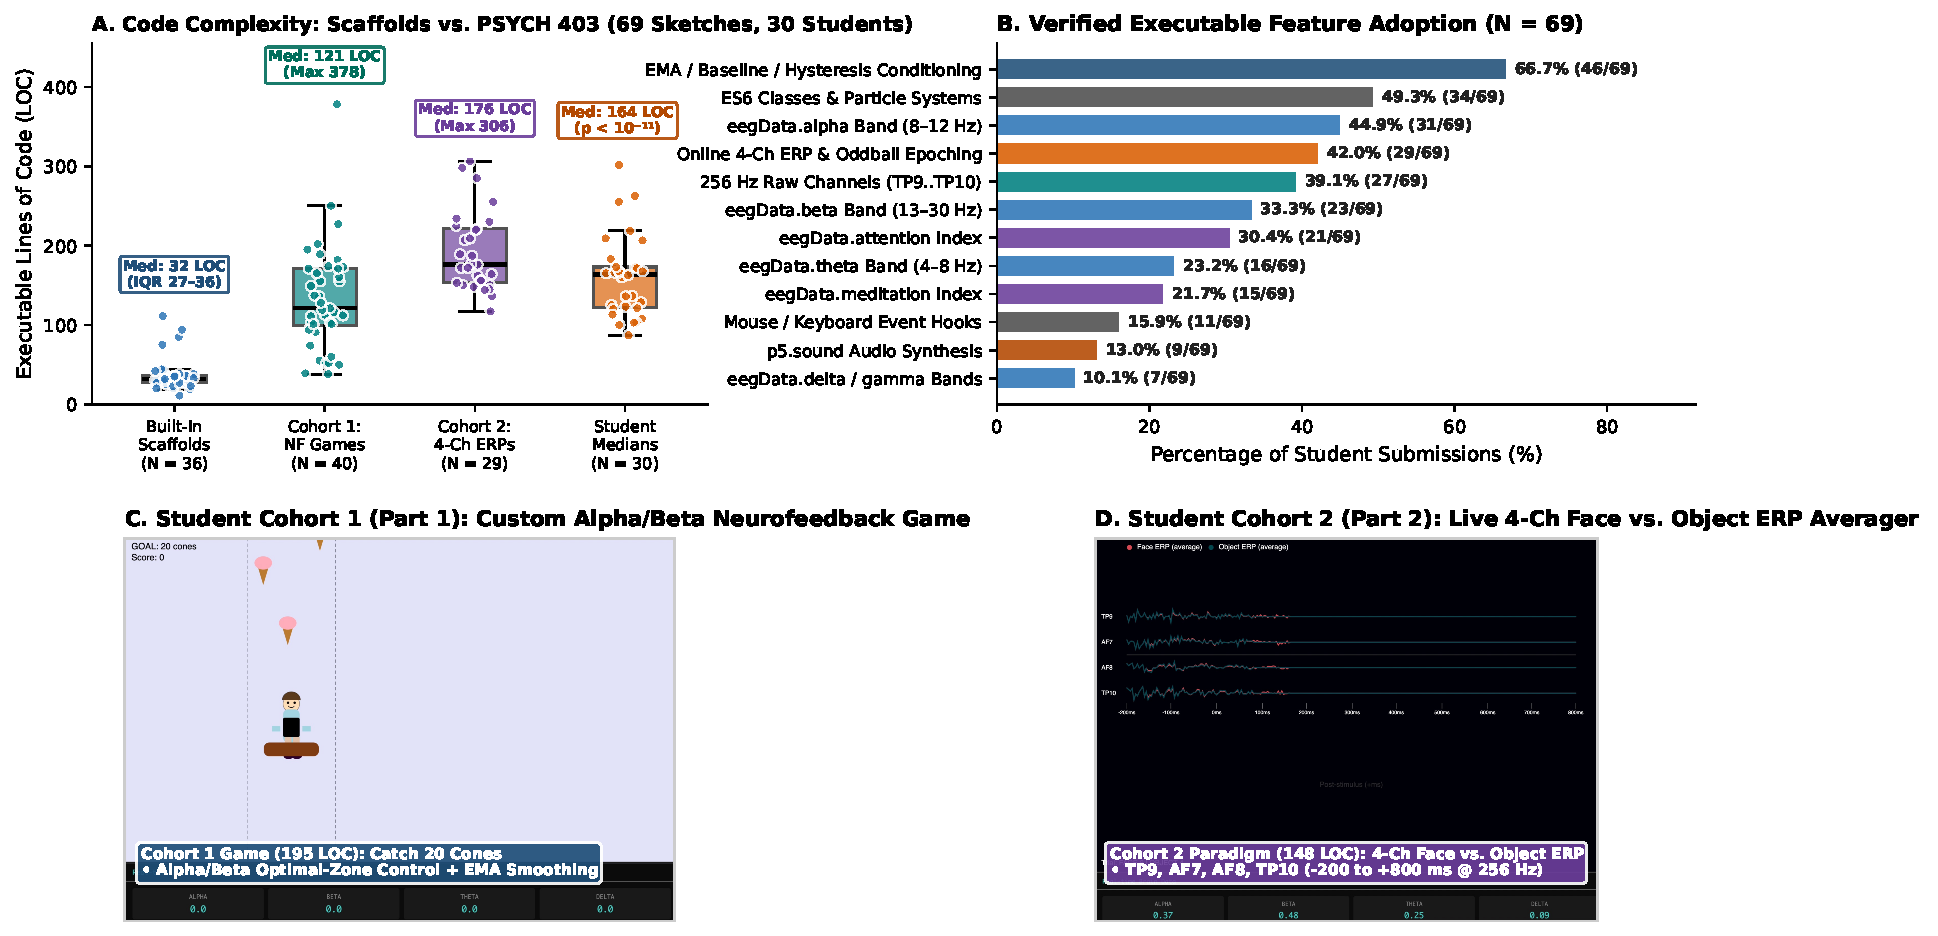
\includegraphics[width=0.98\textwidth]{figures/fig4_psych403_student_submissions_analysis.pdf}
\caption{\textbf{Empirical Evaluation of $N = \NStudentSketches$ Undergraduate Student BrainImation Submissions from $N_{\text{students}} = \NUniqueStudents$ Unique Learners in \texttt{PSYCH 403}.} \textbf{(A)} Executable Lines of Code (LOC) comparing BrainImation's built-in pedagogical scaffolds ($N = \NBuiltinExamples$, median $\ExLOCMedian\text{ LOC}$) against Student Cohort~1 (Continuous Neurofeedback, Art \& Closed-Loop Games; $N = \NStuNF$ sketches, median $\StuNFLOCMedian\text{ LOC}$, max $\StuNFLOCMax\text{ LOC}$), Student Cohort~2 (Online 4-Channel ERP \& Oddball Averagers; $N = \NStuERP$ sketches, median $\StuERPLOCMedian\text{ LOC}$, max $\StuERPLOCMax\text{ LOC}$), and participant-clustered student medians ($N_{\text{students}} = \NUniqueStudents$ independent learners, median $\StuClusterLOCMedian\text{ LOC}$, $p < 10^{-11}$). \textbf{(B)} Verified executable adoption rates of closed-loop signal conditioning, EEG features, experimental paradigms, and \texttt{p5.js} capabilities across all $N = \NStudentSketches$ student programs. \textbf{(C)} Representative Cohort~1 submission (Midterm Part~1, Participant~S14) showing a custom closed-loop neurofeedback game (\emph{Catch 20 Cones}, 195~LOC) driven by live \texttt{ALPHA}/\texttt{BETA} optimal-zone control. \textbf{(D)} Paired Cohort~2 submission (Midterm Part~2, Participant~S14) showing a student-authored 4-channel (\texttt{TP9}, \texttt{AF7}, \texttt{AF8}, \texttt{TP10}) online Face vs.\ Object event-related potential (ERP) averager (148~LOC, $-200\text{ ms}$ to $+800\text{ ms}$ at 256~Hz).}
\label{fig:students}
\end{figure*}

To evaluate how undergraduate psychology and neuroscience students---the vast majority entering without prior JavaScript or digital signal processing experience---use BrainImation in an authentic classroom setting, we analyzed the complete archive of verified unique student code submissions ($N = \NStudentSketches$ \texttt{p5.js} sketches authored by $N_{\text{students}} = \NUniqueStudents$ unique students) from an upper-level undergraduate cognitive neuroscience laboratory course (\texttt{PSYCH 403}, University of Alberta, approved by the University of Alberta Research Ethics Board, Protocol \texttt{Pro00050069}; \textbf{Table~\ref{tab:corpus}} and \textbf{Figure~\ref{fig:students}}). During the course, students first completed guided laboratory sessions exploring frequency-band mappings and oscillatory feedback before authoring two individual programmatic assessments: an open-ended continuous neurofeedback application or game (Midterm Part~1 / Assignment~2; Cohort~1) and an online 4-channel event-related potential experiment built upon raw 256~Hz electrode buffers (Midterm Part~2 / Final Project; Cohort~2). Students developed and debugged their code outside class using \texttt{EEGSimulator} on their personal laptops and tested live closed-loop execution with physical Muse~2 and Muse~2016 headsets during laboratory sessions.

\subsection{Code Complexity Expansion Across Sketch-Level and Participant-Clustered Analyses}
Across all $N = \NStudentSketches$ verified unique submissions, students wrote a median of \StuLOCMedian~executable lines of code ($\text{mean} = \StuLOCMean \pm \StuLOCSD\text{ LOC}$, $\text{IQR} = \StuLOCIQRLow\text{--}\StuLOCIQRHigh\text{ LOC}$, range $\StuLOCMin\text{--}\StuLOCMax\text{ LOC}$)---nearly five times the length of BrainImation's \ExLOCMedian-LOC built-in scaffolds ($U = \MannWhitneyU$, $p < 10^{-15}$, Mann--Whitney $U$ test; \textbf{Figure~\ref{fig:students}A}). Because each student submitted multiple assignments across the semester (typically both a Cohort~1 neurofeedback sketch and a Cohort~2 ERP paradigm), we also performed a strict participant-clustered analysis by collapsing repeated submissions into a single median LOC per unique student ($N_{\text{students}} = \NUniqueStudents$ independent learners). At the independent participant level, student median code complexity remained nearly fivefold larger than the built-in scaffolds at $\StuClusterLOCMedian\text{ LOC}$ ($\text{IQR} = \StuClusterLOCIQRLow\text{--}\StuClusterLOCIQRHigh\text{ LOC}$, range $87\text{--}302\text{ LOC}$; participant-clustered Mann--Whitney $U = \MannWhitneyClusterU$, $p < 10^{-11}$, rank-biserial correlation $r_{rb} = \RankBiserialClusterR$).

Disaggregating the archive by assignment paradigm illustrates how learners elaborated both tracks of the scaffold curriculum. In Student Cohort~1 (Continuous Neurofeedback, Generative Art, and Closed-Loop Games; $N = \NStuNF$, $\text{median} = \StuNFLOCMedian\text{ LOC}$, $\text{IQR} = \StuNFLOCIQRLow\text{--}\StuNFLOCIQRHigh\text{ LOC}$, range $\StuNFLOCMin\text{--}\StuNFLOCMax\text{ LOC}$), students started from 11--38~LOC visual scaffolds and authored complete closed-loop neurofeedback video games and multi-state trainers (\textbf{Figure~\ref{fig:students}C}). Notable student creations include an \emph{EEG Flappy Bird with Adaptive Beta Difficulty} (160~LOC, where alpha power above $0.35$ triggers wing lift while 4-second averaged beta power dynamically scales pipe gap width across 5 difficulty tiers), an \emph{Ice Cream Cone Catcher with Alpha/Beta Optimal Zone Guide} (195~LOC; \textbf{Figure~\ref{fig:students}C}), and a \emph{4-Lane Hysteresis Neurofeedback State Classifier} (378~LOC, implementing 2~s short-term vs.\ 8~s baseline ring buffers, dual-threshold eyes-closed alpha detection $T_{\text{hi}}=1.25 / T_{\text{lo}}=1.05$, and 1.2~s hysteresis state holds).

In Student Cohort~2 (Online 4-Channel ERP and Oddball Paradigms; $N = \NStuERP$, $\text{median} = \StuERPLOCMedian\text{ LOC}$, $\text{IQR} = \StuERPLOCIQRLow\text{--}\StuERPLOCIQRHigh\text{ LOC}$, range $\StuERPLOCMin\text{--}\StuERPLOCMax\text{ LOC}$), students expanded the 85-LOC \texttt{epochs.js} scaffold more than twofold to engineer multi-condition event-related potential paradigms with automated state-machine stimulus schedulers (\texttt{baseline} $-200\text{ to }0\text{ ms}$ $\rightarrow$ \texttt{stimulus} $\rightarrow$ \texttt{postStim} $0\text{ to }+800\text{ ms}$ at $f_s = 256\text{ Hz}$), pre-stimulus baseline subtraction, and separate condition-specific grand-average buffers across \texttt{TP9}, \texttt{AF7}, \texttt{AF8}, and \texttt{TP10} (\textbf{Figure~\ref{fig:students}D}). Student ERP paradigms spanned visual P300 target versus standard oddball tasks, Face versus Object N170 category-selectivity paradigms (\textbf{Figure~\ref{fig:students}D}), Color-Word Stroop conflict tasks, and auditory Mismatch Negativity (MMN) designs.

\subsection{Verified Executable Signal Conditioning, EEG Modality, and Paradigm Adoption}
To avoid inflating feature counts with comment strings or generic canvas variables (such as RGBA color opacity named \texttt{alpha} or 2D game paddle boundary clamping), we restricted our automated code inspection strictly to non-comment executable lines referencing explicit \texttt{eegData} properties and neural conditioning operations (\textbf{Figure~\ref{fig:students}B}). Two-thirds of all student submissions ($\StuPctCond\%$, $\StuCntCond/\NStudentSketches$ sketches) implemented explicit closed-loop neural signal conditioning, including first-order EMA recursion ($\hat{y}_t = \lambda\hat{y}_{t-1} + (1-\lambda)x_t$), linear interpolation (\texttt{lerp()}) on EEG state variables, pre-stimulus baseline subtraction, or hysteresis hold counters to stabilize live neural control. Across structural paradigms, $\StuPctParticles\%$ ($\StuCntParticles/\NStudentSketches$) defined custom ES6 \texttt{class} structures or dynamic particle arrays, $\StuPctERP\%$ ($\StuCntERP/\NStudentSketches$) implemented online multi-trial ERP or oddball epoching state machines, and $\StuPctEvents\%$ ($\StuCntEvents/\NStudentSketches$) integrated custom keyboard, mouse, or DOM slider hooks. Across explicit \texttt{eegData} modalities, students combined \texttt{eegData.alpha} ($\StuPctAlpha\%$, $\StuCntAlpha/\NStudentSketches$; $77.5\%$ of Cohort~1 neurofeedback sketches), 256~Hz \texttt{raw}/\texttt{getRecentEpoch} electrode channels ($\StuPctRaw\%$, $\StuCntRaw/\NStudentSketches$), \texttt{eegData.beta} ($\StuPctBeta\%$, $\StuCntBeta/\NStudentSketches$), \texttt{eegData.attention} ($\StuPctAtt\%$, $\StuCntAtt/\NStudentSketches$), \texttt{eegData.theta} ($\StuPctTheta\%$, $\StuCntTheta/\NStudentSketches$), \texttt{eegData.meditation} ($\StuPctMed\%$, $\StuCntMed/\NStudentSketches$), and \texttt{p5.sound} Web Audio synthesis ($\StuPctAudio\%$, $\StuCntAudio/\NStudentSketches$).

\section{Discussion}
\textsc{BrainImation} establishes a self-contained, constructionist live-coding environment for accessible neurotechnology and experimental electrophysiology. While it pairs naturally with guided electrophysiology dashboards such as \emph{EEGEdu} (\url{https://eegedu.com}) \citep{mathewson2026eegedu} that introduce how bioelectrical potentials are amplified, filtered, and transformed into frequency spectra, BrainImation operates as a standalone browser IDE that empowers researchers, students, and artists to use live neural signals as a programmable medium \citep{papert1980mindstorms,resnick2009scratch,deleeuw2015jspsych}. By solving the Muse~2 and Muse~S lazy GATT characteristic advertisement bug in a \MuseBrowserKB~KB zero-dependency WebBluetooth module, exposing a dual-source \texttt{window.eegData} state contract backed by a 256-point Hanning-windowed FFT and a 256~Hz 4-channel physiological simulator, dynamically auto-binding \texttt{p5.js} and \texttt{p5.sound}, and embedding a \NRefAPIs-primitive snippet-injecting reference panel alongside serverless URL portfolio loading, BrainImation removes the multi-language software engineering barrier that previously separated domain specialists from active BCI and ERP development.

Several technical, physiological, and methodological considerations qualify our findings and inform experimental best practices. First, because WebBluetooth packets arrive in 12-sample ($46.875\text{ ms}$) bursts and browser rendering loops operate asynchronously at the display refresh rate ($60\text{ Hz}$, $16.67\text{ ms}$ per frame), software-stamped stimulus triggers in browser-based ERP paradigms (\texttt{epochs.js} and Cohort~2 student sketches) incur $\sim 15\text{--}45\text{ ms}$ of latency jitter relative to hardware TTL triggers \citep{krigolson2017choosing,kuziek2017transitioning,kuziek2018increasing}. While this jitter acts as a temporal low-pass filter that attenuates sharp early sensory potentials, broader endogenous components such as the visual N170 and oddball P300 remain resolvable within 20 averaged trials ($\text{SNR} = \ERPSNRKTwenty$; \textbf{Figure~\ref{fig:sonification}C} and \textbf{Figure~\ref{fig:students}D}), and analyzing this timing trade-off provides a transparent demonstration of real-time acquisition engineering. Second, dry-electrode consumer headbands positioned over anterior frontal (\texttt{AF7}, \texttt{AF8}) and temporo-parietal (\texttt{TP9}, \texttt{TP10}) sites are highly susceptible to ocular blinks (EOG) and frontalis or temporalis muscle tension (EMG) \citep{lotte2013flaws,mathewson2017high}. Although \texttt{MuseEEGManager} screens out gross $>150\ \mu\text{V}$ amplitude transients prior to FFT computation and \texttt{EEGSimulator} injects explicit bilateral frontal blinks so users can test artifact thresholding, practitioners should note that forehead beta/gamma power can still reflect subtle facial muscle tension and that posterior alpha modulation is best captured at \texttt{TP9}/\texttt{TP10} during eyes-closed relaxation. Third, regarding cross-browser portability, only Chromium-based browsers (Google Chrome, Microsoft Edge, and Opera on desktop/Android, or the Bluefy WebBluetooth browser on iOS/iPadOS) currently implement the W3C WebBluetooth API required for physical Muse pairing; however, \texttt{EEGSimulator} and the entire Monaco, WebGL, and Web Audio IDE execute natively in Apple Safari and Mozilla Firefox, ensuring universal hardware-free development on any personal computer. Finally, our empirical human-factors evaluation quantified executable code complexity and feature adoption across $N = \NStudentSketches$ program artifacts rather than pre- and post-course psychometric tests, and users had access to both built-in scaffolds and optional AI coding tools (\texttt{AIAssistant}), meaning lines of code reflect overall application scope rather than unaided syntax recall. As demonstrated by our $N_{\text{students}} = \NUniqueStudents$ novice cohort, equipping users with a zero-install browser IDE and \ExLOCMedian-line scaffolds enables rapid design, debugging, and serverless sharing of closed-loop neurofeedback games, multi-band audio synthesizers, and online 4-channel ERP experiments entirely inside a standard web browser.

\subsection*{Declarations}
\noindent\textbf{Ethics Statement:} Classroom code artifacts from \texttt{PSYCH 403} were analyzed in de-identified form in accordance with procedures approved by the University of Alberta Research Ethics Board (Protocol \texttt{Pro00050069}).\\[2pt]
\noindent\textbf{Data and Code Availability:} The live \textsc{BrainImation} IDE is freely accessible at \url{https://kylemath.github.io/Brainimation/}. Complete open-source source code (\texttt{muse-browser.js}, \texttt{index.html}, and all 36 scaffold sketches in \texttt{examples/}) and reproducible analysis and figure-generation scripts are permanently archived at \url{https://github.com/kylemath/Brainimation} and \url{https://github.com/kylemath/eegeduPaper}.\\[2pt]
\noindent\textbf{Funding:} This work was supported by a Natural Sciences and Engineering Research Council of Canada (NSERC) Discovery Grant to K.E.M.\\[2pt]
\noindent\textbf{Declaration of Competing Interest:} The author declares no competing financial or non-financial interests.\\[2pt]
\noindent\textbf{CRediT Authorship Contribution Statement:} \textbf{Kyle E. Mathewson:} Conceptualization, Methodology, Software, Validation, Formal analysis, Investigation, Data curation, Writing -- original draft, Writing -- review \& editing, Visualization, Supervision.

\bibliographystyle{apalike}
\bibliography{references2}

\end{document}
